\documentclass[draftclsnofoot,onecolumn,letterpaper,10pt]{IEEEtran}
\pagestyle{empty}
\usepackage{geometry}
\geometry{textheight=9.5in, textwidth=7in}

\usepackage{float}
\usepackage{graphicx}
\usepackage{algorithm2e}

\newcommand{\subparagraph}{}
\usepackage{titlesec}

\titleformat{\section}[block]{\bfseries\Large}{\thesection}{0.4em}{}
\titleformat{\subsection}[block]{\bfseries\large}{\thesubsection}{0.4em}{}
\titleformat{\subsubsection}[block]{\bfseries\normalsize}{\thesubsubsection}{0.4em}{}
\setlength{\parindent}{0pt}
\renewcommand{\thesection}{\arabic{section}}
\renewcommand{\thesubsection}{\thesection.\arabic{subsection}}
\renewcommand{\thesubsubsection}{\thesubsection.\arabic{subsubsection}}



\date{\today}

\title{brew.ai Design Document}

\begin{document}
{\huge\textbf{Senior Software Engineering Design Group 7}}
	\vspace{1cm}

{\Huge\textbf{brew.ai Design Document}}

\vspace{2cm}
\textbf{Connor Yates} yatesco@oregonstate.edu

\textbf{Aravind Parasurama} parasura@oregonstate.edu

\textbf{Cody Holliday} hollidac@oregonstate.edu

\vspace{2cm}
Sponsor

Dale McCauley, College of Business, Oregon State University

\vspace{0.5cm}
	Approved: 

	Version: 1.0


\newpage
\begin{abstract}
	Home beer or mead brewing is not currently a process as simple as brewing coffee.
	We aim to change this, and make home brewing as easy as brewing coffee with the OpenBrew project.
	The OpenBrew project will consist of two major components:
	A hardware system for physically automating the brewing process, and a software system for managing the brewing process, utilizing machine learning 
		to optimize mead or beer recipes.
	Through these components, a user will be able to easily incorporate a fully automated, intelligent home brewing system into an existing setup or 
		as the framework to construct a new brewing system.
\end{abstract}
\newpage
\tableofcontents
\newpage
\section{Introduction}
% Perhaps get rid of these subsection titles, and just combine it into one larger section with appropriate paragraph spacings.
% These talk about the Purpose, scope, etc, of this paper.
brew.ai is a hardware and software solution for automated brewing of mead or beer. Currently, home brewing requires a lot of time, knowledge, and 
	patience. 
As such, it is not accessible to amateurs, and brew.ai attempts to solve this problem. 
From amateurs to professional brewers, we want brew.ai to be useful in automating the brewing process, and helping brewers make better tasting products. 
The brew.ai device itself is a bucket lid that will fit over a brewing device and have various modules incorporated in it. 
The lid device will monitor and control temperature, send and receive commands/data to and from the Android application, and monitor fermentation status.
Improving recipes will take place in the back-end, in the form of a service that the Android software will communicate with. 
As a user, setup will simple and essentially plug-and-play. 
No technical knowledge is needed beyond knowing how to pair a bluetooth bucket lid with an Android device.

\subsection{Purpose}
This document describes the architecture and design of the brew.ai project.
It conforms to the IEEE 1016 System Design Document specification, and lays out the design of hardware, learning, and android interfaces for the project.

\subsection{Scope}
Stated generally, brew.ai is a device which automatically brews fermented drinks and improves its performance over time based on user feedback.
This allows for users 
\subsection{Context}
\subsection{Overview}


\section{Glossary}

\section{Stakeholders and Design Concerns}
% Here we list out the design concerns of stakeholders (users, etc...) that we address in this document.
% By laying out the design concerns now, we can address each in turn in the subsequent design sections.

\section{System Overview}

\section{Design Viewpoints}
% Details each design point we choose for this project.
% The tech review had 3 technologies, with 3 choices/investigations for each tech.
% Each of the three technologies chosen should be designed in detail in its own "viewpoint".
% each viewpoint then has its own "view". There can be more than one of these.
% the views describe the specific implementations that each viewpoint covers. Refer to the doc for more info.

\subsection{Abstract Learning from Previous Trials} %connor's
From the inception, a major component of this project is the idea that it can learn from mistakes and experiments, and improve the quality of the brew over time.
This section looks at the system design from the viewpoint of artificial intelligence creation.
From this perspective, all other design choices of the project are abstracted into general data sources and sinks.
To further illustrate this point, the view Impact on Other Designs, in Section~\ref{sec:AIImpact}, will introduce the reader to this viewpoint by describing its view of the rest of the system.
From there, the AI system's internal view of the brew.ai system will be explained and designed.

\subsubsection{Impact on Other Designs}\label{sec:AIImpact}
From the viewpoint of learning, the two other major viewpoints, electronic hardware and user interfaces, have little to no impact upon the operations of the system.
There will be interaction between these viewpoints, but that does not imply the other sections will autonomously impact the operation of the system.

From the AI perspective, the system is built as a thinking agent, with the ability to send and receive signals.
This allows the agent to change the world it sees (input signals) through its actions (sent signals).
The hardware will be the main component the AI will interact with, as it provides information about the world through sensors, and can change the world through its actuators.
From this perspective, the hardware is generalized into the two categories: sensors and actuators.
This is a common view for an agent to take in regards to its interaction with the world~\cite{RussellNorvig}.
A diagram summarizing the agent's view of the system is presented in Figure~\ref{fig:AIsystemDesign}.

\begin{figure}\label{fig:AIsystemDesign}
\begin{center}
	\caption{brew.ai System Heirarchy from the viewpoint of the agent}
	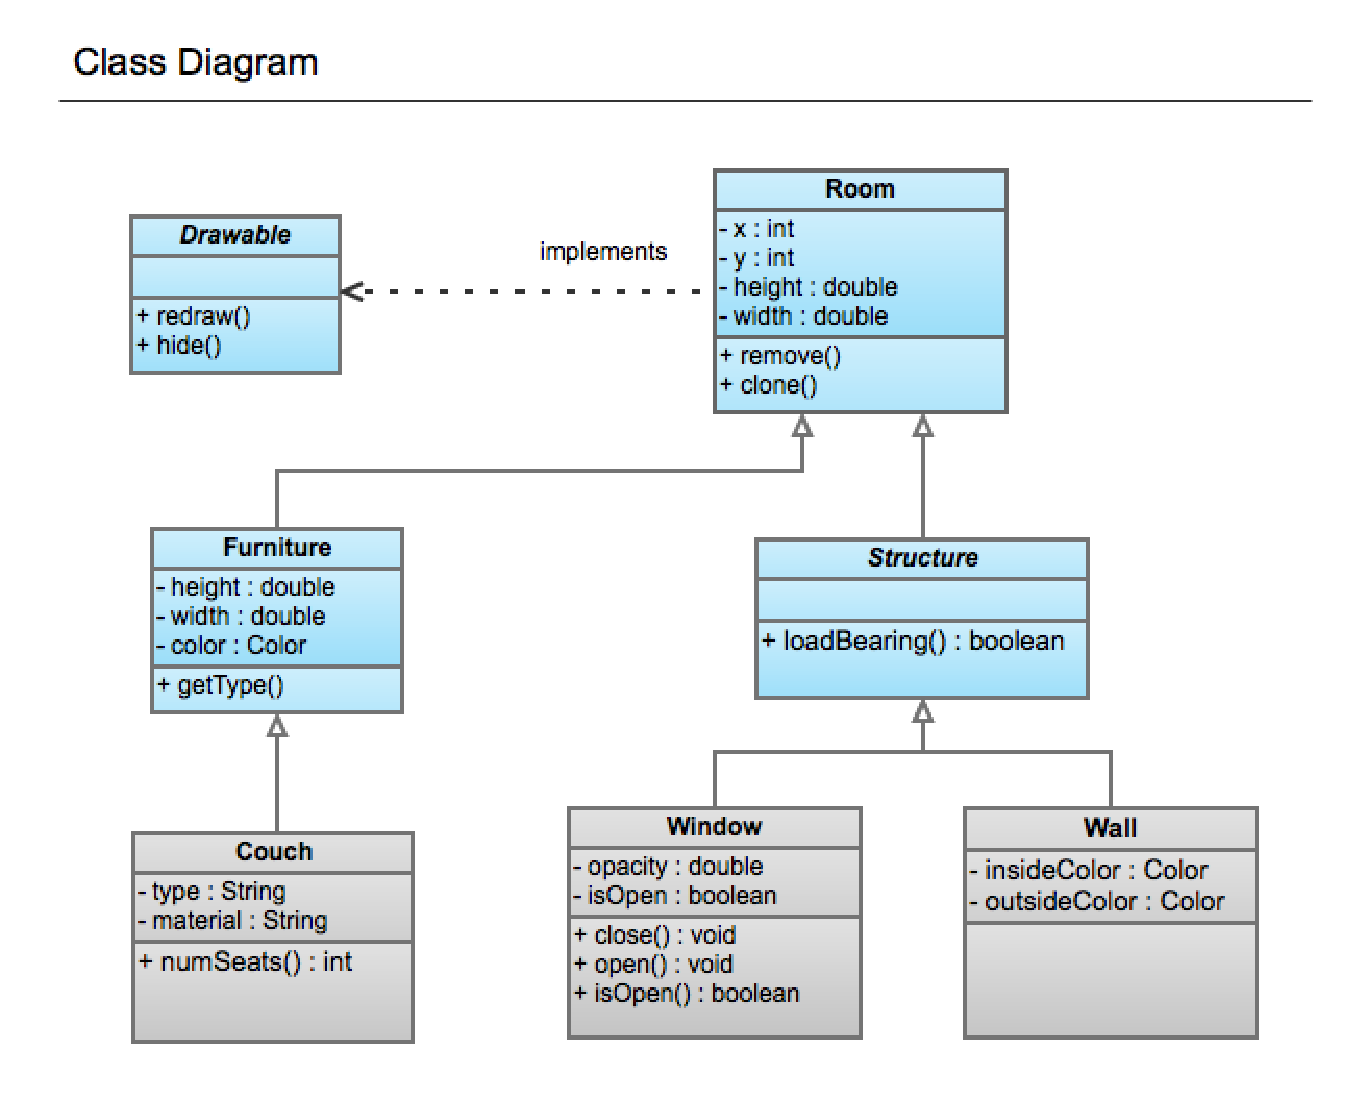
\includegraphics[scale=0.3]{tmp.eps}
\end{center}
\end{figure}

The agent will also view the user interface as source of actuators and sensors, but this will be limited in scope.
The main task of the agent is to brew drinks, not report information to the user.
Therefore, the main decision-making processes will focus on the hardware interaction (reading sensor values, changing temperature levels, etc.) and not on intelligent interaction with the user.
The direct interaction between the user and the AI will be limited to sending statistical information for display, and basic controls such as start-stop controls.

A standard communication layer will be necessary to communicate between the AI, hardware, and interface.
This will be implemented with standard protocols and library packages, such as JSON for interface communication, and byte streams for hardware interaction.
Builtin Python libraries exist for these communication protocols, and subsequently will be used.

\subsubsection{Learning Algorithm} 
% talk about what algorithm I chose.
% Any design considerations that this algorithm requires
% design of this piece, in the context of the project
The agent will be using standard Q-learning, as it provides a proven framework for creating intelligent agents that can learn

Q-learning design

Agent state design

Agent action design

\subsubsection{Decision Making Structures}
An important aspect of intelligent decision making is the computational structure which allows for decisions to be made.
Neural networks are a classic method of non-linear function approximation~\cite{RussellNorvig},  which we will use to approximate the Q-table.
This can be done by collapsing the state into a single dimensional vector, and using this as the input to the neural net.
The neural net will output the Q-value associated with each action for this state, which are used by the Q-learning as normal, if they came from a Q-table.


\begin{algorithm}[H]\label{alg:Qlearning}
	\caption{Q-Learning Standard Algorithm}
	statement in Algorithm

\end{algorithm}


\textbf{describe neural network structure}
Input layer, hidden layer, output layer, activation function

In order to train the neural network to approximate the Q-table, backpropagation will be used along with a sum-of-squares loss function.
Methods such as backpropogation are standard entries in neural-network and machine learning libraries, which we will use to provide the implementation.

If the neural network structure does not provide reliable performance, then we will use a traditional Q-table to implement the learning.
The reason this is not used by default is because we have a continuous state space, which cannot be contained in a finite table.
However, by observing the incoming data, we can provide an encoding scheme which will map the continuous domain of data inputs into a finite, discrete set which can be used to construct the table.


\begin{figure}\label{fig:nn}
\begin{center}
	\caption{Proposed Neural Network Structure}
	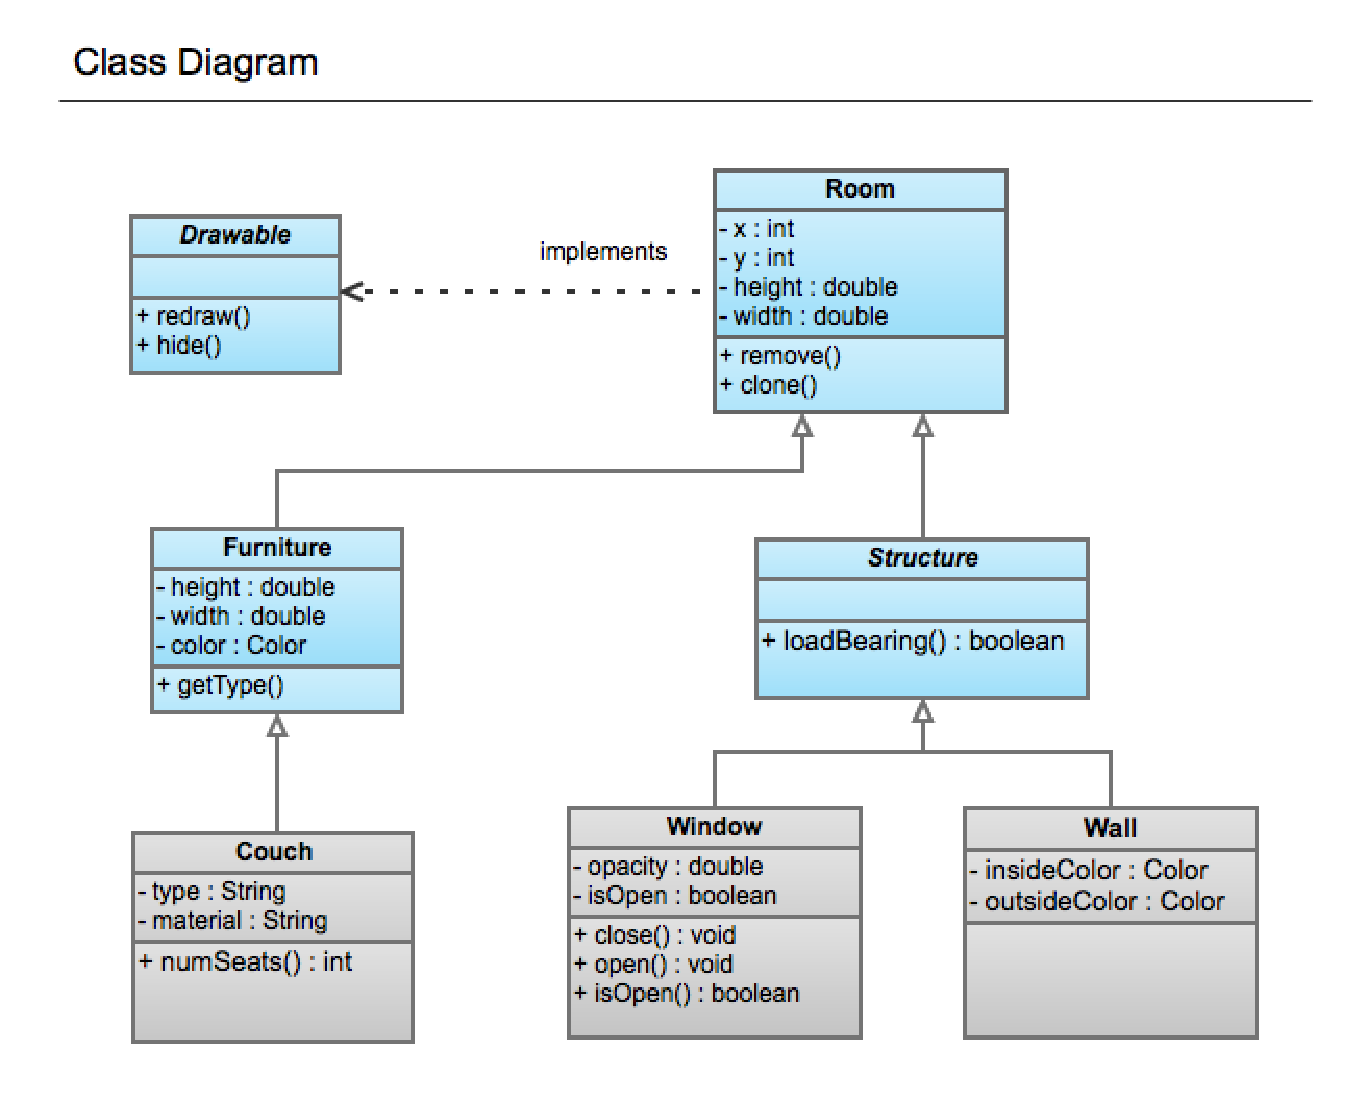
\includegraphics[scale=0.3]{tmp.eps}
\end{center}
\end{figure}

\subsubsection{Overall Agent Structure}
This section will tie together the designs laid out previously, and provide a total system diagram for the agent.

\begin{figure}\label{fig:AgentStructure}
\begin{center}
	\caption{Agent structure, showing learning functions, neural network, and data insertion points}
	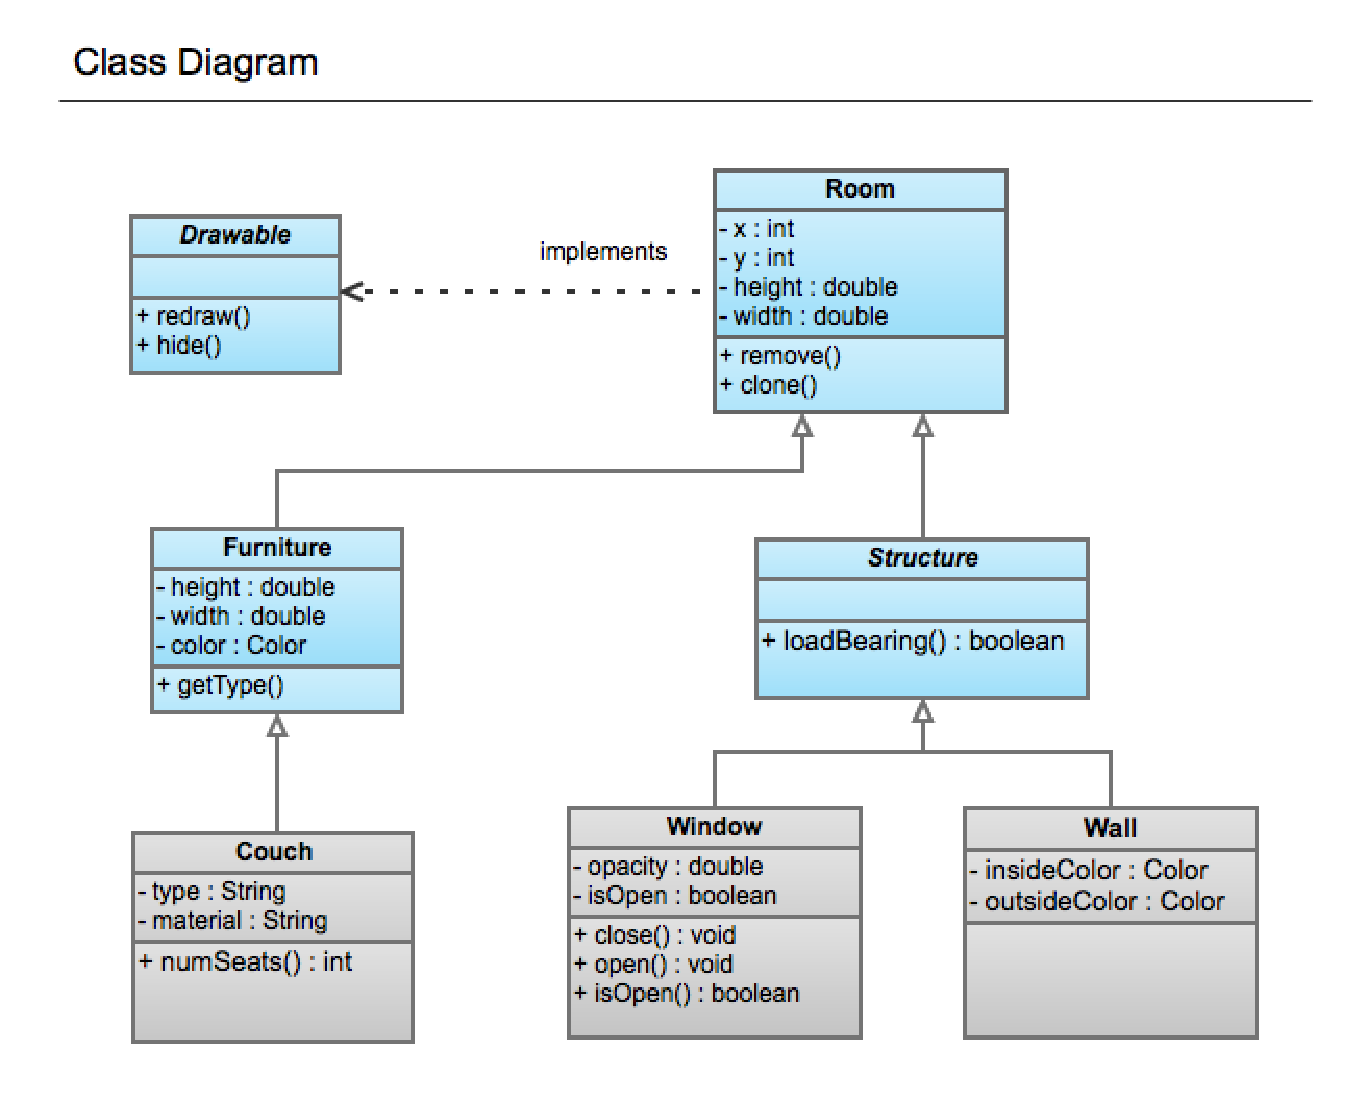
\includegraphics[scale=0.3]{tmp.eps}
\end{center}
\end{figure}

\subsection{Android-Based User Interface Design} %cody's
\subsubsection{Interface Device}

\subsubsection{UI Connection to controller}

\subsubsection{Dataflow to UI}

\subsubsection{Interface layout}


\subsection{Brewing Hardware and Electronic Controls} %aravind's section
The brewing hardware is expected to perform the commands received from the Android client, while also automatically managing
some basic regulation functions on its own. The hardware will collect data about the brewing process and relay that back to the
Android application.

\subsubsection{Temperature control implementations}
For temperature control, a peltier junction will be used, attached to a heatsink on one side. The temperature control module will
hang from the lid of the device, and touch the liquid so as to apply a temperature differential to the liquid itself. Peltier junctions 
operate with pulse-width modulation, and at the levels of current required, an H-BRIDGE will have to be utilized in conjunction with the 
peltier module.

\subsubsection{Data collection from brewing process}
For data collection, an array of sensors has been chosen:
\begin{enumerate}
	\item A thermocouple, for minimal calibration temperature data gathering
	\item A carbon dioxide sensor, for measuring current fermentation levels
	\item A digital hydrometer for measuring initial gravity
\end{enumerate}
\subsubsection{Hardware connection to the client}
Data will be transmitted to the front-end by means of bluetooth. A bluetooth module will be used that supports interfacing directly with AVR's
USART functionality. This bluetooth module should easily pair with the Android application and transfer data.

\subsubsection{Central control system}
To bring all of the hardware components together, we will be using the Teensy 2.0, powered by the ATmega32u4. This microcontroller allows for basic
routines to be performed, and has a variety of hardware functionality that will be extensively used in this project.

\section{Design Rationale}

\section{Testing Details and Timeline}
% Reuse gantt chart for project timeline, and specify where testing would take place in that chart.
% Add details for testing your own components, and potentially testing interactions with other components.

\section{Summary}

% References
\bibliography{design_document}
\RestyleAlgo{boxed}
\bibliographystyle{ieeetr}


\end{document}
